\chapter{Introduction}
\label{sec:introduction}
\todo{
    * **Introduction**\\
    * Ruff problem description\\
    * How \ac{ABE} can solve this\\
    * How \ac{ABE} works\\
    * Short history summary of \ac{ABE}\\
    * What is expected of this work\\
    * What are the targets
}
In public-key cryptography each user is identified by his unique public and private key pair. Peer-to-peer communication works well with this scheme, but as soon as an encrypted content needs to be accessed by multiple participants, the data owner has to encrypt the content for each user explicitly. This results in many encrypted versions of the same  file, each secured by a different public key. Such schemes do not scale well in the secure cloud storage domain. Here often data owners want to share the same content with many other users at the same time.

The point is reached where the classical public-key end-to-end encryption scheme does not scale anymore. To overcome this obstacle an encryption scheme need to be employed which has a constant number of access keys regardless of the number of participants.
\todo{extend}

\section{Secure Cloud Storage System}
In the past 20 years we witnessed a shift of resource consumption on the user side to outsourcing more and more resources into the cloud. Naturally, users moved their files into cloud storage systems. This helped companies to maintain an ecosystem around the user helping him to synchronize his files onto different devices.  

With increasing transparency raised also the concern that it was not clear anymore who could access the private files especially when they are transmitted and stored on oversee servers. Bdrive, a secure cloud storage system, committed to not export files and data to other countries. It splits up files in smaller chunks that are saved separately on different cloud storage provider (\ac{CSP}). To ensure end-to-end encryption a Bdrive client encrypts locally each of its chunks with a one-time symmetric key that is then encrypted under its own public key. This encrypted key is called a file key and it is uploaded to the Bdrive server where it is stored securely, as shown in figure \ref{fig:filekey}.

\section{Background}
\begin{figure*}[!ht]
\centering
    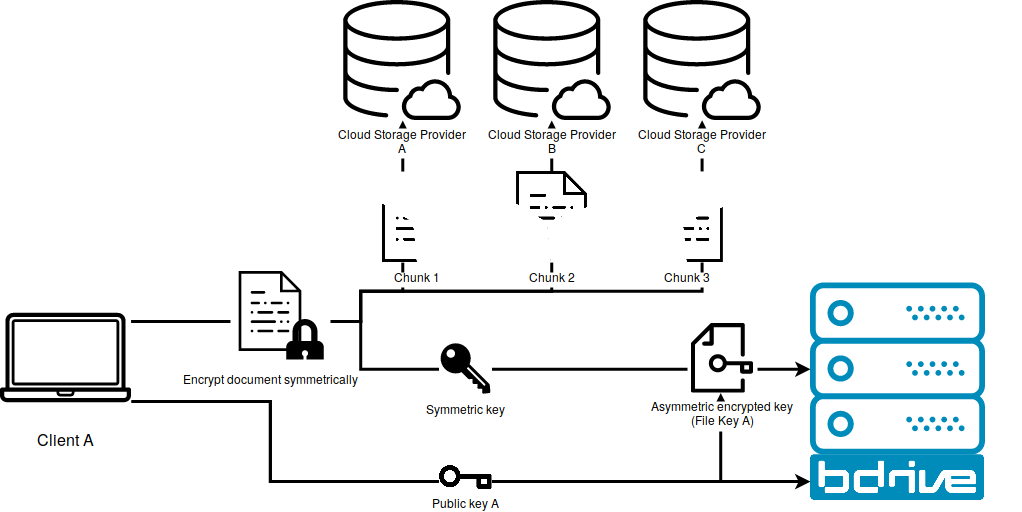
\includegraphics[width=0.8\linewidth]{img/bdrive1.png}\par 
    \caption{Device uploads an encrypted file to the \ac{CSP}s and the file key and public key to Bdrive.}
    \label{fig:filekey}
\end{figure*}
\begin{figure*}[!ht]
\centering
    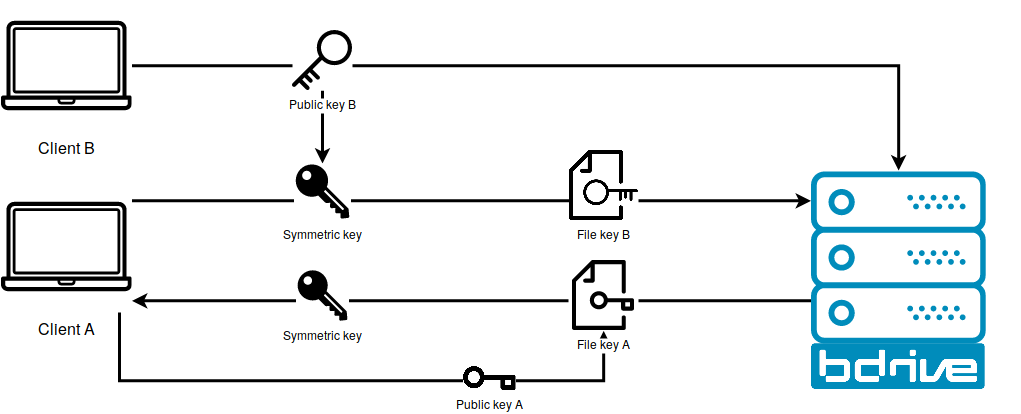
\includegraphics[width=0.8\linewidth]{img/bdrive2.png}\par
    \caption{Device A grants Device B access to the uploaded file by re-keying the file key}
    \label{fig:rekey}
\end{figure*}
Since each device of the same user has its own private-public key pair, an existing device is in charge of making its accessible file keys available for a new device. This will be done by downloading each file key for the respective file, receiving the public key of the new device, decrypting the file key with its own private key, encrypting it again with the public key of the new device and finally, uploading the new file key to the Bdrive server. This process will be called re-keying, as shown in figure \ref{fig:rekey}. 

% File upload and file key creation
In Bdrive each device of a user generates a new \ac{RSA} key pair on registration. The fingerprint (SHA-1 or MD5 hash) of the public key identifies the device uniquely. To save a file in the cloud the device first encrypts the file symmetrically with the so called "filekey". The filekey equals the hash of the plain file content and so ensures tamperproofness and integrity on decryption. End-to-end encryption implies that the server should never be able to decrypt the file by itself. To enforce this the device encrypts the filekey asymmetrically with its own public key before uploading the filekey to the Bdrive server where it is stored securely. In Bdrive, the encrypted file chunks are uploaded to the different cloud storage provider (\ac{CSP}). 

% Access file
If the user wants to access a file locally, the devices requests the encrypted filekey from the server and downloads the file chunks from the \ac{CSP}s. Locally, it decrypts the filekey with his private key and finally deciphers the assembled file with the decrypted filekey. 

% Process for multibe devices
So far the encryption process for a single device has been outlined. However, this process turns out to be much more computationally complex in a multiple device setting.  If a user registers more then one device the existing data needs to be synchronized to the new device. The server notifies the existing device for the newly registered one and the public key of the new device is downloaded. Now the existing device needs to download each filekey for each file of the user and decrypts it. The synchronization is finished by encrypting the filekeys with the new devices public key and uploaded again to the server. The new device can now start to download and decrypt the file chunks as described previously.

Usually in cloud storage systems we also have the concept of groups. They describe a collection of clients which share data between them. For that they form a so called \textit{share}. To express the overhead of joining or leaving a share the following notation will be used: $f$ and $n$ donate the number of filekeys and the number of devices in a share respectively.

% Adventages
If a new devices joins a share in Bdrive a device needs to make the existing file keys available to the new devices which results in $f$ additional encryptions, messages and keys. However, a big advantage of this scheme is that forward secrecy\footnote{Forward Secrecy: The left entity will have no knowledge about future shared content.} will not produce additional overhead. Here, only all the filekeys belonging to the left device are removed and the other devices do not further encrypt new uploaded files for this device anymore. The backward secrecy constrain, while being an imported security feature, will explicitly be broken by clients. This is due to the feature, that data owner can invite a new member into a group and the new member accesses all previous uploaded content. Bdrive is ensuring this by explicitly reencrypting all file keys for the new device. 

\section{Problem Description}
% Bdrive rekeying
% Motivation and Problem description

% Disadventages in shares
Notice, that this approach is not scalable for a large number of devices. To showcase this, the use case of creating a new share is analyzed. Each device invited to a share needs to have an own version of the file key, encrypted with the devices public key, issued. This process scales with $O(n * f)$ keys. 
%Were $n$ donates the number of devices involved in the sharing and $f$ the number of file versions in the share.\footnote{Each file consist of many file versions. Each file version needs an own file key since for each content change a new file is updated.}
Further, the same number of messages containing the encrypted file key need to be send and each filekey needs to be encrypted $n$ times which also results in $O(n * f)$ encryptions in total. 

To make the overhead more clear, lets assume a manager of a company with 50 employees who wants to create a company wide share. Each of the employees has at least two devices (say one web view client and a desktop client). To upload the latest presentation the device of the manager know has to create $50 * 2 = 100$ filekeys to upload, $100-1$ messages, containing encrypted file key for each device, to distribute and $100$ encryptions to make. Even worst for each new presentation upload another $100$ filekeys need to be maintained. In a large scale company this overhead becomes unmaintainable when the number of $10.000$ filekeys are exceeded. \footnote{Running 'openssl speed rsa1024' on an Intel(R) Core(TM) i7-6500U CPU @ 2.50GHz takes on average 0.000113s for encryption. Multiplied by 10.000 the second mark is reached.} With increasing computing power this problem can be compensated but not prevented.

\section{Attribute-Based encryption}
\textit{Attribute-Based Encryption} (\ac{ABE}) defines users over attributes and attribute keys rather then its individual public key. Since users are not unique among their attribute set it is possible to reduce the number of needed keys of a share to the number of attributes necessary to describe the group completely. 

In the previous example the manager would only need to encrypted the presentation one time: With the public key of the attribute “working in company”. In this participial use case only $1$ encryption is done, $1$ message is distributed using multi-cast to transmit same encrypted file to all clients, and $1$ file key is created. 

Of cause this advantage does come at some cost. While classical encryption schemes provide complete End-to-End encryption, ABE needs a \textit{Attribute Authority} (\ac{AA}) to issue attribute and attribute keys in the first place. This authority has global decryption power in the administered domain. For that reason the attributes need to be split up into different domains, each managed by an own AA. In the use case of cloud storage systems for business it makes sense to setup an AA for each company. 

With ABE comes the advantage of defining access policies for cipher texts. This policies consist of boolean formulas with attribute values as inputs. Only if a user satisfies the given policy he is able to decipher the cipher text. The use of this access formulas helps to eliminate authorization checks, since clients can either decrypt the file and are therefor allowed to access the plaintext or they are not able to decrypt and so do not satisfy the given policy. 

% In our use case inter company sharing becomes tricky. Now different AAs need to cooperate to create cipher text policies containing attributes of the whole ecosystem.  

ABE scales with the number of attributes contained in a cipher text. As long as a group can be described with less attributes then there are members in this group, a better performance of ABE compared to the current scheme in Bdrive can be achieved. 

\section{Contribution}
In this work different schemes suitable to resolve the rekeying problem will be compared. First, the group communication schemes on a theoretical bases are compared. Then it is argued why ABE might scale even better and different schemes are compared on a practical level. To do so a homogeneous platform was used and different benchmarks will be performed to evaluate the performance and scalability of thous schemes. Thous benchmarks are novel in that matter that no other research compared the different ABE topics on a practical level.  

In the second part of this work, an prototype implementation of the selected approach will be given which will stay as close as possible to the current scheme in Bdrive. To make the selected scheme practically applicable and to fit the requirements of section \ref{sec:requirements}, small adaptation to the scheme will be made. The target will be to compare the current scheme and the ABE approach. Further, a conclusion of the applicability of ABE in the real world is drawn and it is evaluated whether ABE does also scale better in real life scenarios. 